\section{Simulation Analysis}
\label{sec:simulation}

	Tables~\ref{tab1:npn} and~\ref{tab1:pnp}  shows the voltages required to confirm that the BJTs are operating Forawrd Active Region (F.A.R), 
by comparing $V_{CE}$ and $V_{BE}$ for the NPN transistor and $V_EC$ and $V_EB$ for the PNP. Analysing the results, we can confirmar that, in fact,
the BJTs do operate in F.A.R.

\begin{table}[H]
  \centering
  \begin{tabular}{|l|r|}
    \hline    
    {\bf Voltages} & {\bf V} \\ \hline
    \input{../sim/npn_tab}
  \end{tabular}
  \caption{NPN Voltages and F.A.R confirmation}
  \label{tab1:npn}
\end{table}

\begin{table}[H]
  \centering
  \begin{tabular}{|l|r|}
    \hline    
    {\bf Voltages} & {\bf V} \\ \hline
    \input{../sim/pnp_tab}
  \end{tabular}
  \caption{PNP Voltages and F.A.R confirmation}
  \label{tab1:pnp}
\end{table}


Regarding the simulation results, we present them below in Table~\ref{tab1:sim}.
Note that, in the previous section, we presented this results to compare to the theoretical
ones.

\begin{table}[H]
  \centering
  \begin{tabular}{|l|r|}
    \hline    
    {\bf Name} & {\bf V or dB} \\ \hline
    \input{../sim/sim_tab}
  \end{tabular}
  \begin{tabular}{|l|c|}
    \hline
    {\bf Impedance} & {\bf kOhms} \\ \hline
    zin & 2.236262e+00\\ \hline

  \end{tabular}
  \begin{tabular}{|l|c|}
    \hline
    {\bf Impedance} & {\bf kOhms} \\ \hline
    \input{../sim/output_tab}
  \end{tabular}
    \caption{Simulation Results.}
    \label{tab1:sim}
\end{table}

It is important, in order to guarantee a high compatibility with AUDIO IN and speakers, that we obtain a very high input impedance ($Z_I$) and a very low output impedance ($Z_O$). Analysing our results, we notice that despite having a small input impedance (in result of a compromise we had to make to obtain a higher merit figure), the output impedance is very low, as desired.




\subsection{Coupling Capacitors}
In order to analyse this circuit, we need to understand the coupling capacitors influence. In this BJT amplifier circuit, there are two couplin capacitors, $C_{in}$ and $C_O$ - because their functions are similar, we will focus only on capacitor $C_{in}$. In the graphics below, we present the frequency response of the circuit, but with $C_{in}$ values drastically differents.

\begin{figure}[h]
\centering
\begin{subfigure}{.5\textwidth}
    \centering
    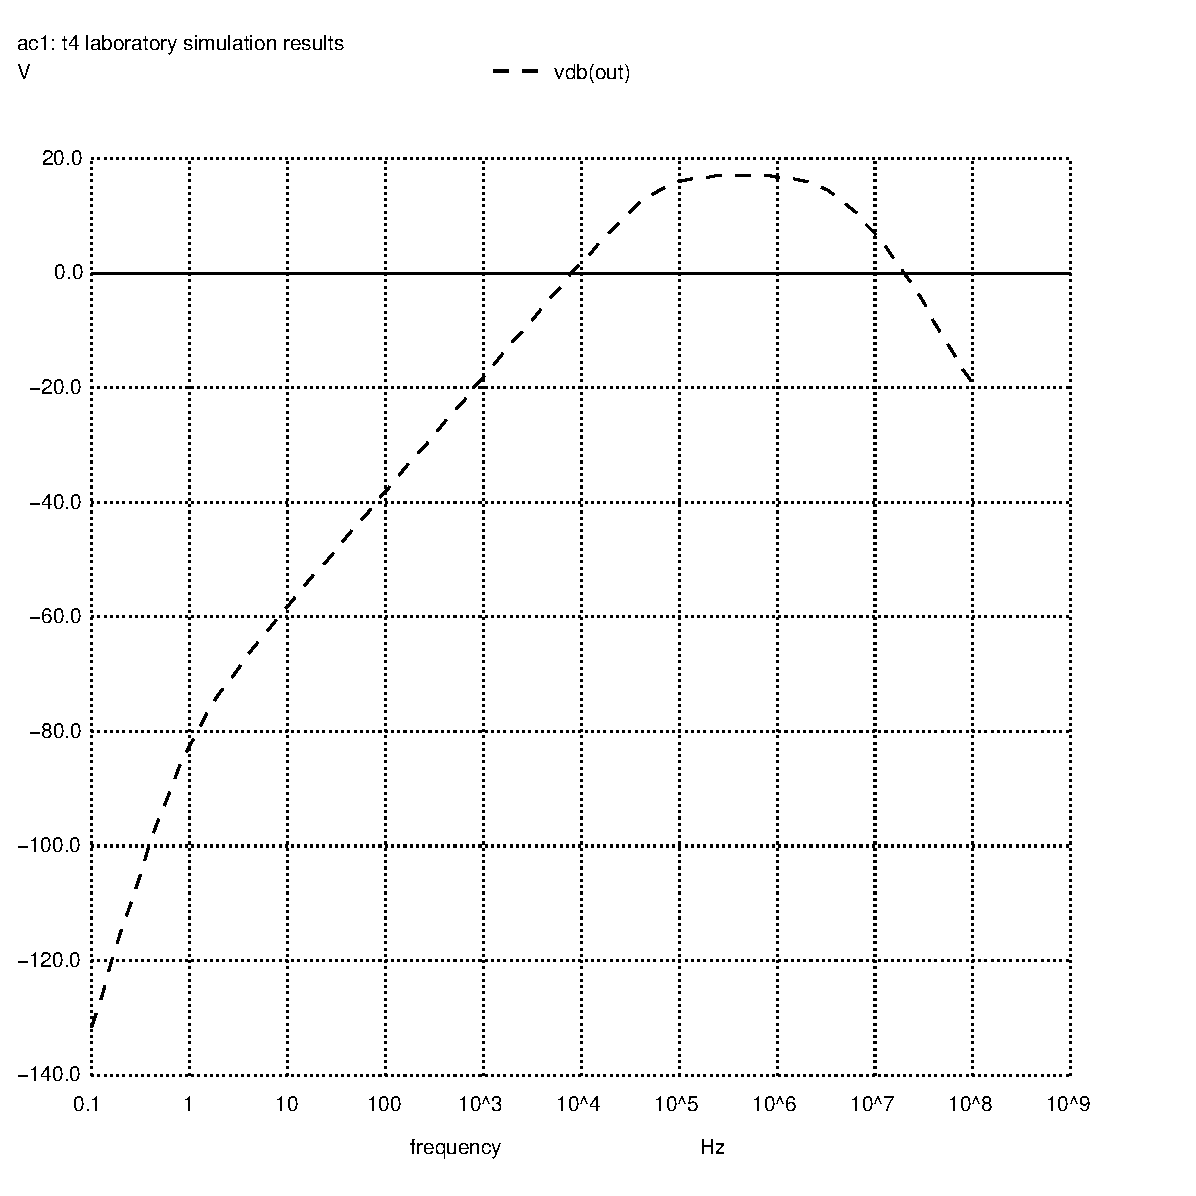
\includegraphics[scale=0.33]{Images/couplingsmall.ps}
    \caption{Low $C_{in}$=1nF}
\end{subfigure}%
\begin{subfigure}{.5\textwidth}
    \centering
    \includegraphics[scale=0.33]{Images/couplingbig.ps}
    \caption{High $C_{in}$=1F}
\end{subfigure}
\caption{$C_{in}$ influence on the frequency response of the circuit.}
\label{fig_coupling}
\end{figure}

As we can notice, the change in the capacitance of the coupling capacitor does not influence the value of the higher cut-off frequency. However, the increase of that value leads to a larger bandwidth, which is desired.

This happenas because, when $\omega \to 0$, $Z(C_{in}) \to \inf$ and, therefore, this capacitor prevents the transistor from entering on the saturation or the cut-off regions, by blocking the DC component of the AUDIO IN source. This helps mantaining the OP of the transistor, so that it can operate at lower frequencies, as $C_{in}$ increases.


\subsection{Bypass Capacitor}
Next, we must analyse the influence of the Bypass Capacitor $C_b$ on the circuit. In the graphics below, we present the frequency response of the circuit, but with $C_b$ values drastically differents.

\begin{figure}[h]
\centering
\begin{subfigure}{.5\textwidth}
    \centering
    \includegraphics[scale=0.33]{Images/bypasssmal.ps}
    \caption{Low $C_E$=1nF}
\end{subfigure}%
\begin{subfigure}{.5\textwidth}
    \centering
    \includegraphics[scale=0.33]{images/bypassbig.ps}
    \caption{High $C_E$=1F}
\end{subfigure}
\caption{$C_E$ influence on the circuit.}
\end{figure}

By placing the bypass capacitor in parallel with $R_E$, this resistor becomes short for medium and high frequencies and because the amplifier's first stage gain is inversely dependent on this resistance, the bypass capacitor helps maximizing the gain for medium and high frequencies, which is desired.


\subsection{Resistor $R_C$}
Finally, we must understand the effect on the circuit of changing $R_C$. In the graphics below, we present the frequency response of the circuit, but with $R_C$ values drastically differents.


\begin{figure}[h]
\centering
\begin{subfigure}{.5\textwidth}
    \centering
    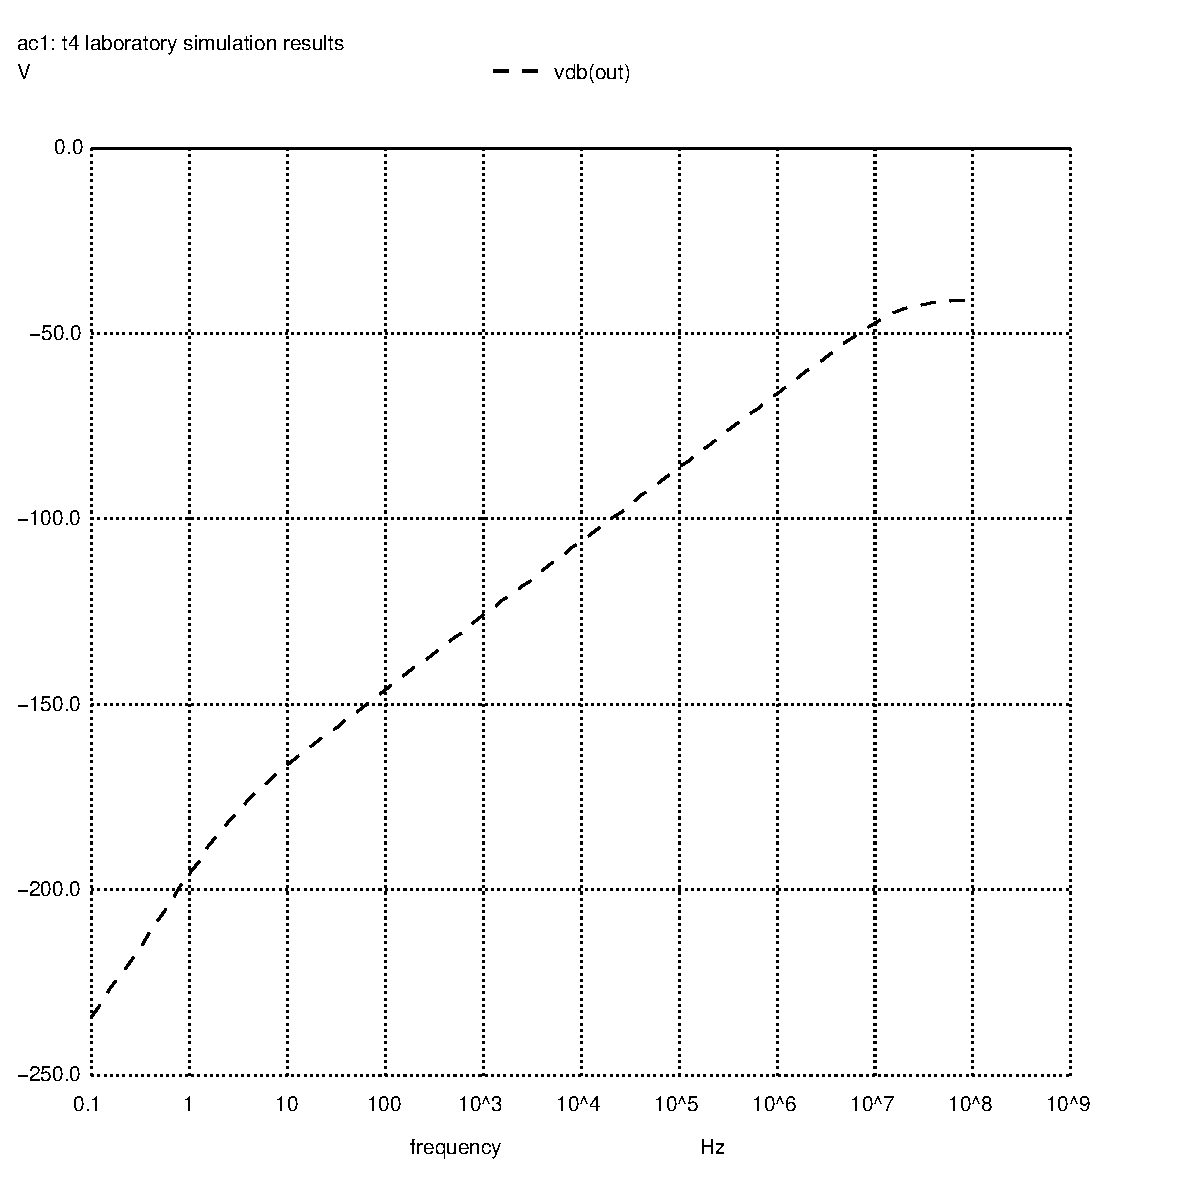
\includegraphics[scale=0.33]{images/rcsmall.ps}
    \caption{Low $R_C$=10$\Omega$}
\end{subfigure}%
\begin{subfigure}{.5\textwidth}
    \centering
    \includegraphics[scale=0.33]{images/rcbig.ps}
    \caption{High $R_C$=10$k\Omega$}
    \label{fig:RC_High}
\end{subfigure}
\caption{$R_C$ influence (on the Gain)}
\end{figure}


As we can notice, when we increase $R_C$, the gain increases and the passaband is antecipated. Note that for high values of resistance, a bizarre graphic is described. 

\subsection{Gain.}
\pagebreak

We are now ready to make a global comparison of the two approaches, with the chosen values for the constants. Below, we present both the theoretical and simulation graphs of the gain:

\vspace{-2.5cm}

\begin{figure}[h]
\centering
\begin{subfigure}{.5\textwidth}
    \centering
    \vspace{2.8 cm}
    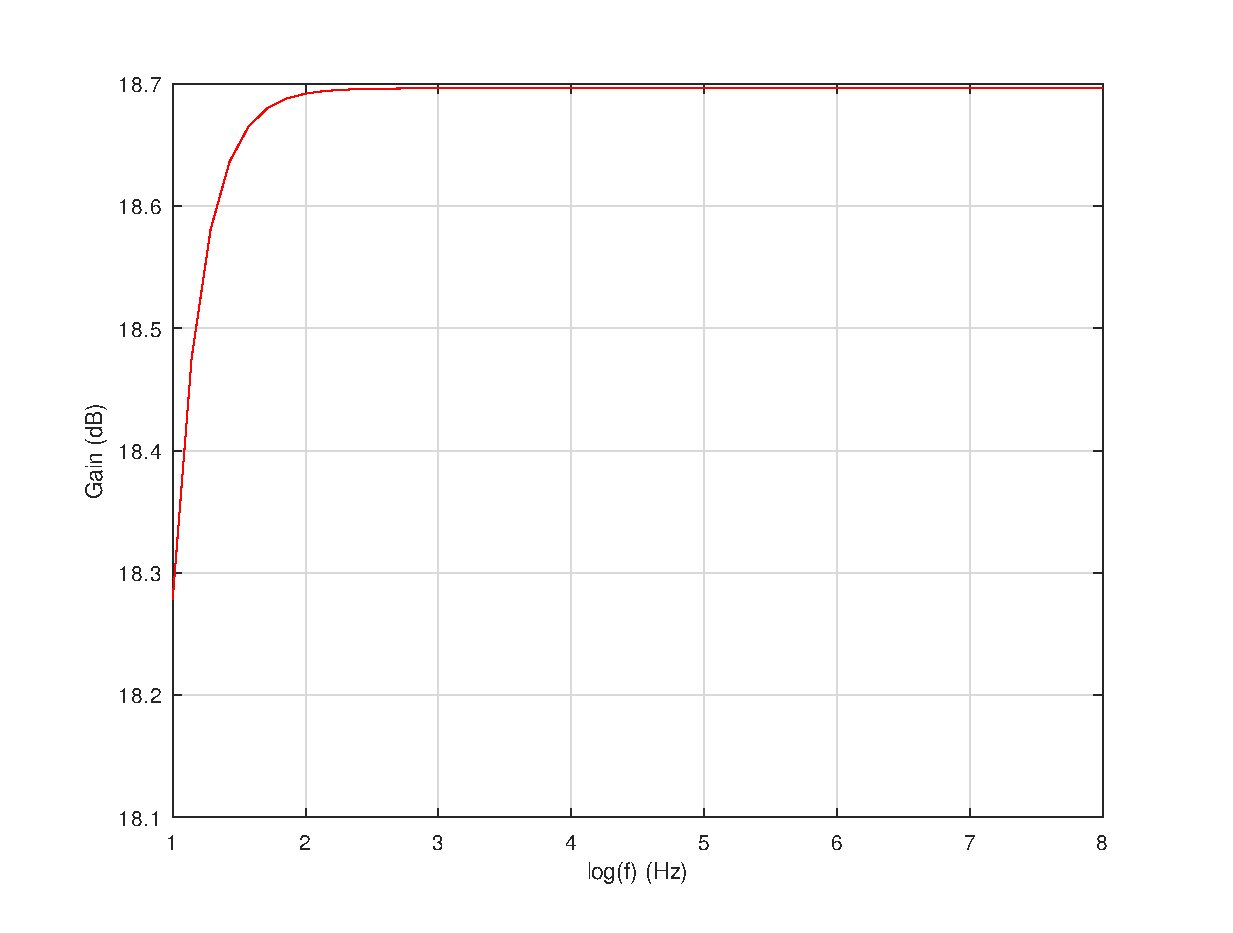
\includegraphics[scale=0.4]{Gain.eps}
    \caption{Theoretical Gain}
\end{subfigure}%
\begin{subfigure}{.5\textwidth}
    \centering
    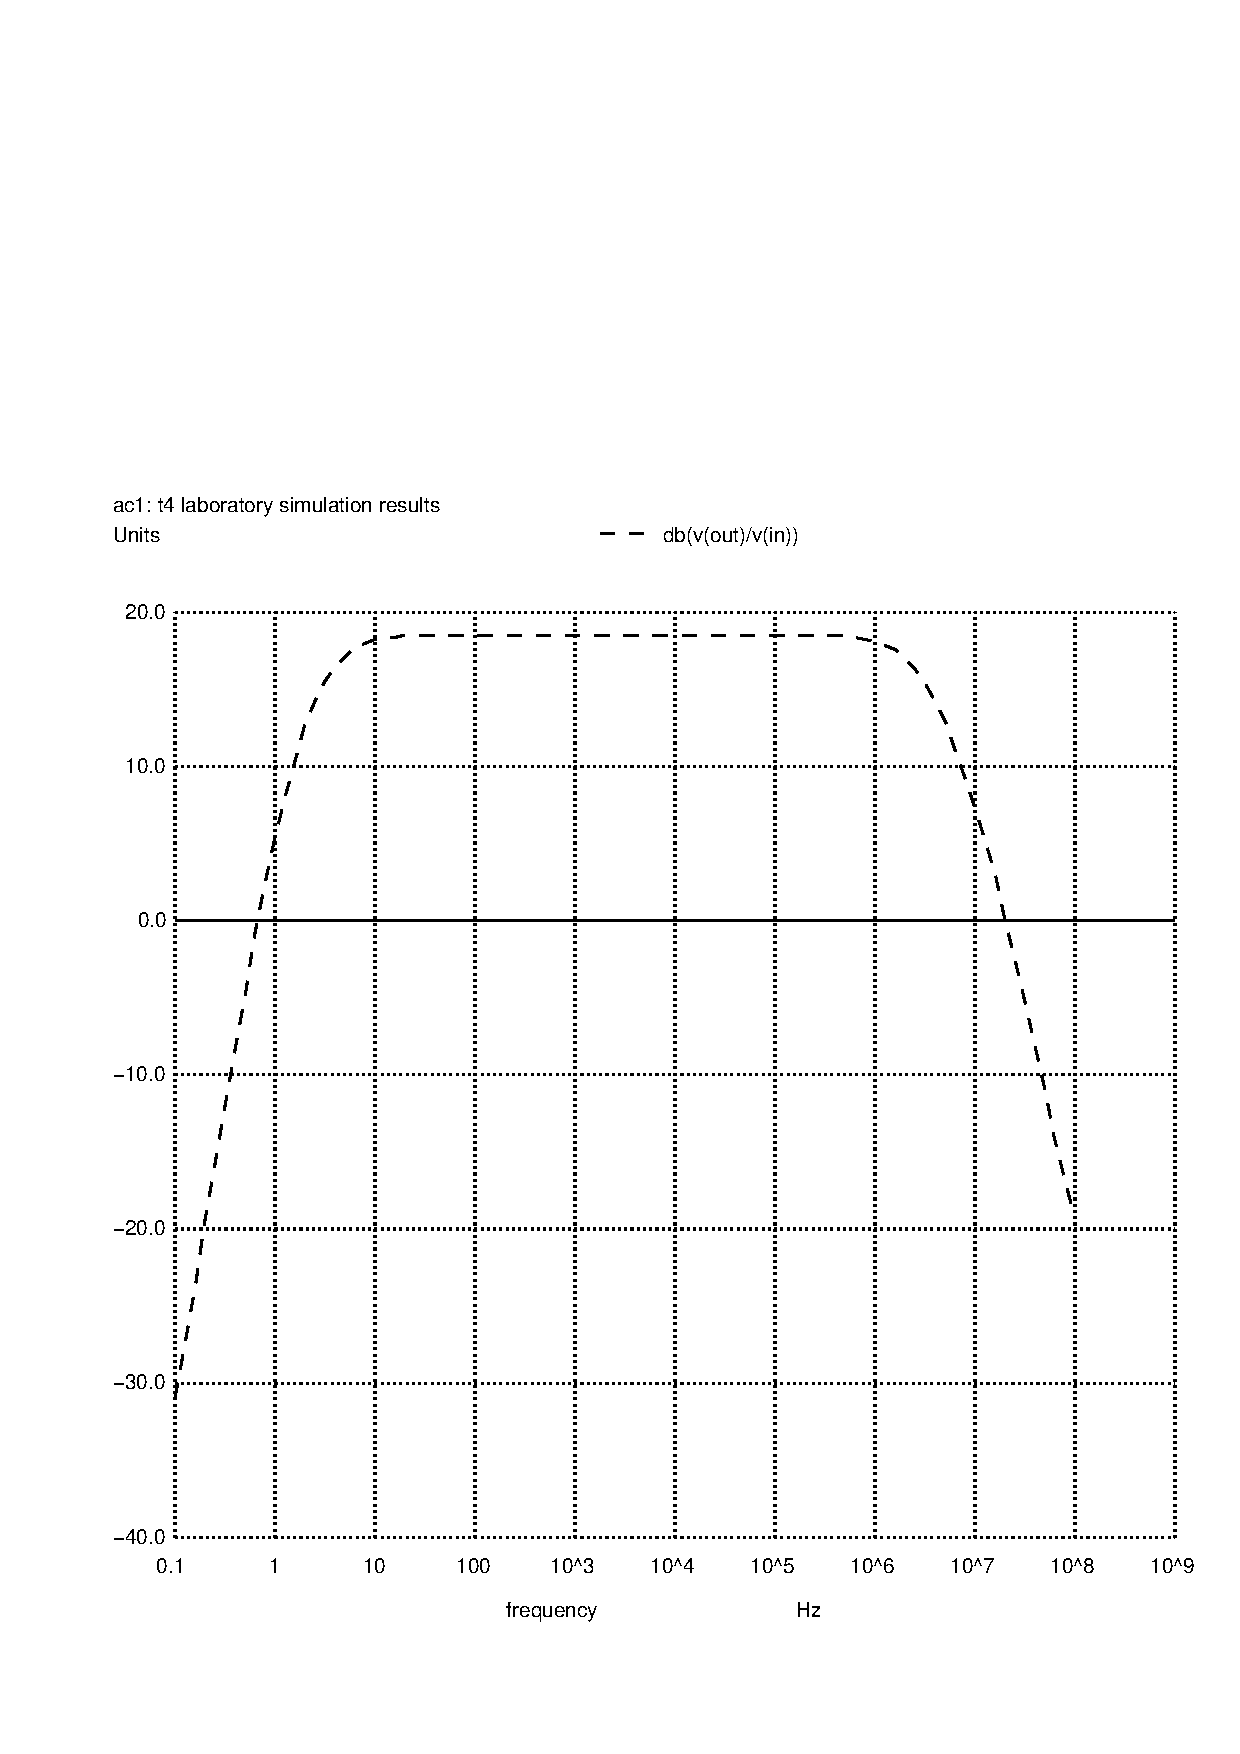
\includegraphics[scale=0.33]{gain.pdf}
    \caption{Simulation Gain}
\end{subfigure}
\caption{Gain}
\label{fig:Gain}
\end{figure}

In this case, the comparison of the shape can only be done on the left side, since we don't have the theoretical higher cut-off frequency. 

Comparing both figures, we can conclude that the overall shape of the graphs is similar, noting that the theoretical curve can be thought of as assymptotical approach. Furthermore, we can see that the Gain and the lower cut-off frequency are quite similar - they may differ slightly because not only the theoretical result is an approximation, as said previously, but the transistors used in the NGSPice were real ones.

Note that the logaritmic scale of the frequency begins in $-1$, not $1$ as requested initially because, by trying to improve the figure of merit, we ended up having a circuit whose low cutoff frequency happened at a frequency lower that the smaller value of the scale.


\subsection{Merit}
To end this section, we outline below the 4 values that influence the merit figure and the respective value of the merit.

\begin{table}[H]
  \centering
  \begin{tabular}{|l|r|}
    \hline    
    {\bf Name} & {\bf Values} \\ \hline
    Gain(dB)&37.0419\\ \hline
Gain& 71.1371\\ \hline
Central Frequency(Hz)& 1051.2\\ \hline
Gain deviation&28.8629\\ \hline
Central frequency deviation(Hz)&51.2041\\ \hline
Cost(MU)& 13446.7\\ \hline
Merit & 9.28821E-07\\ \hline

  \end{tabular}
  \caption{Values for the calculation of the Merit.}
\end{table}

As we can see, we obtained a very high merit value. However, that value was obtained at the cost of degrading the quality of the circuit (for example, the low input impedance.)


